


\begin{frame}{RoboCup 2004}

%\vspace{1em}
\justifying

As an undergraduate I participated in a yearlong {\bf robotics project} in which
we programmed ERS-210 and ERS-7 robotic dogs made by Sony to compete in the 
Standard Platform League (SPL) of the international {\bf RoboCup 2004 competition}.

\vspace{2em}

\twocol{0.5}{
\justifying
Our technical report~\cite{Dahm2004} provides an in-depth look into the core
challenges of teaching robots to play soccer, the solutions developed by our
team, and the involved support infrastructure. 

\vspace{1em}
As part of the GermanTeam -- a collaboration between the universities of Berlin,
Bremen, Darmstadt, and Dortmund -- we won the world championship in the SPL 
as well as the SPL Open Challenge.

}{0.41}{
\vspace{-1.75em}
\begin{figure}
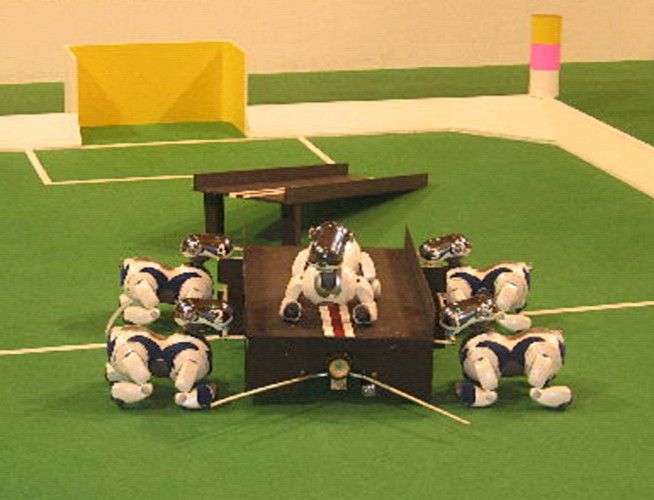
\includegraphics[width=\linewidth]{robocup/robocup.jpg}

\vspace{-1em}
\caption{\scriptsize Scene from the SPL Open Challenge~\cite{Dahm2004}.}
\end{figure}
}

\vspace{1em}

\begin{center}
\rule{2cm}{0.4pt}\\[0.5em]
\end{center}

\fc{Dahm2004}{publications/2004-02/2004-02}

\end{frame}
